\chapter{Závěr}
\label{ch:zaver}

V rámci tohoto semestrálního projektu byla úspěšně navržena a implementována kompletní analytická a deterministická část systému pro automatizované předběžné zpracování astronomických snímků. Systém úspěšně integruje nízkoúrovňové operace pro čtení datových struktur \ac{FITS}, automatizovaný modul pro segmentaci kalibračních dat a matematické subsystémy pro mřížkový odhad pozadí a profilování geometrie hvězd. Spojení vysokovýkonného výpočetního jádra a lehkého reaktivního klientského rozhraní prokázalo vysokou propustnost dat při matematických transformacích pixelů, přičemž celkový přehled o architektuře hotového uživatelského rozhraní je znázorněn na Obrázku~\ref{fig:full_ui_screenshot}.

\begin{figure}[htbp]
    \centering
    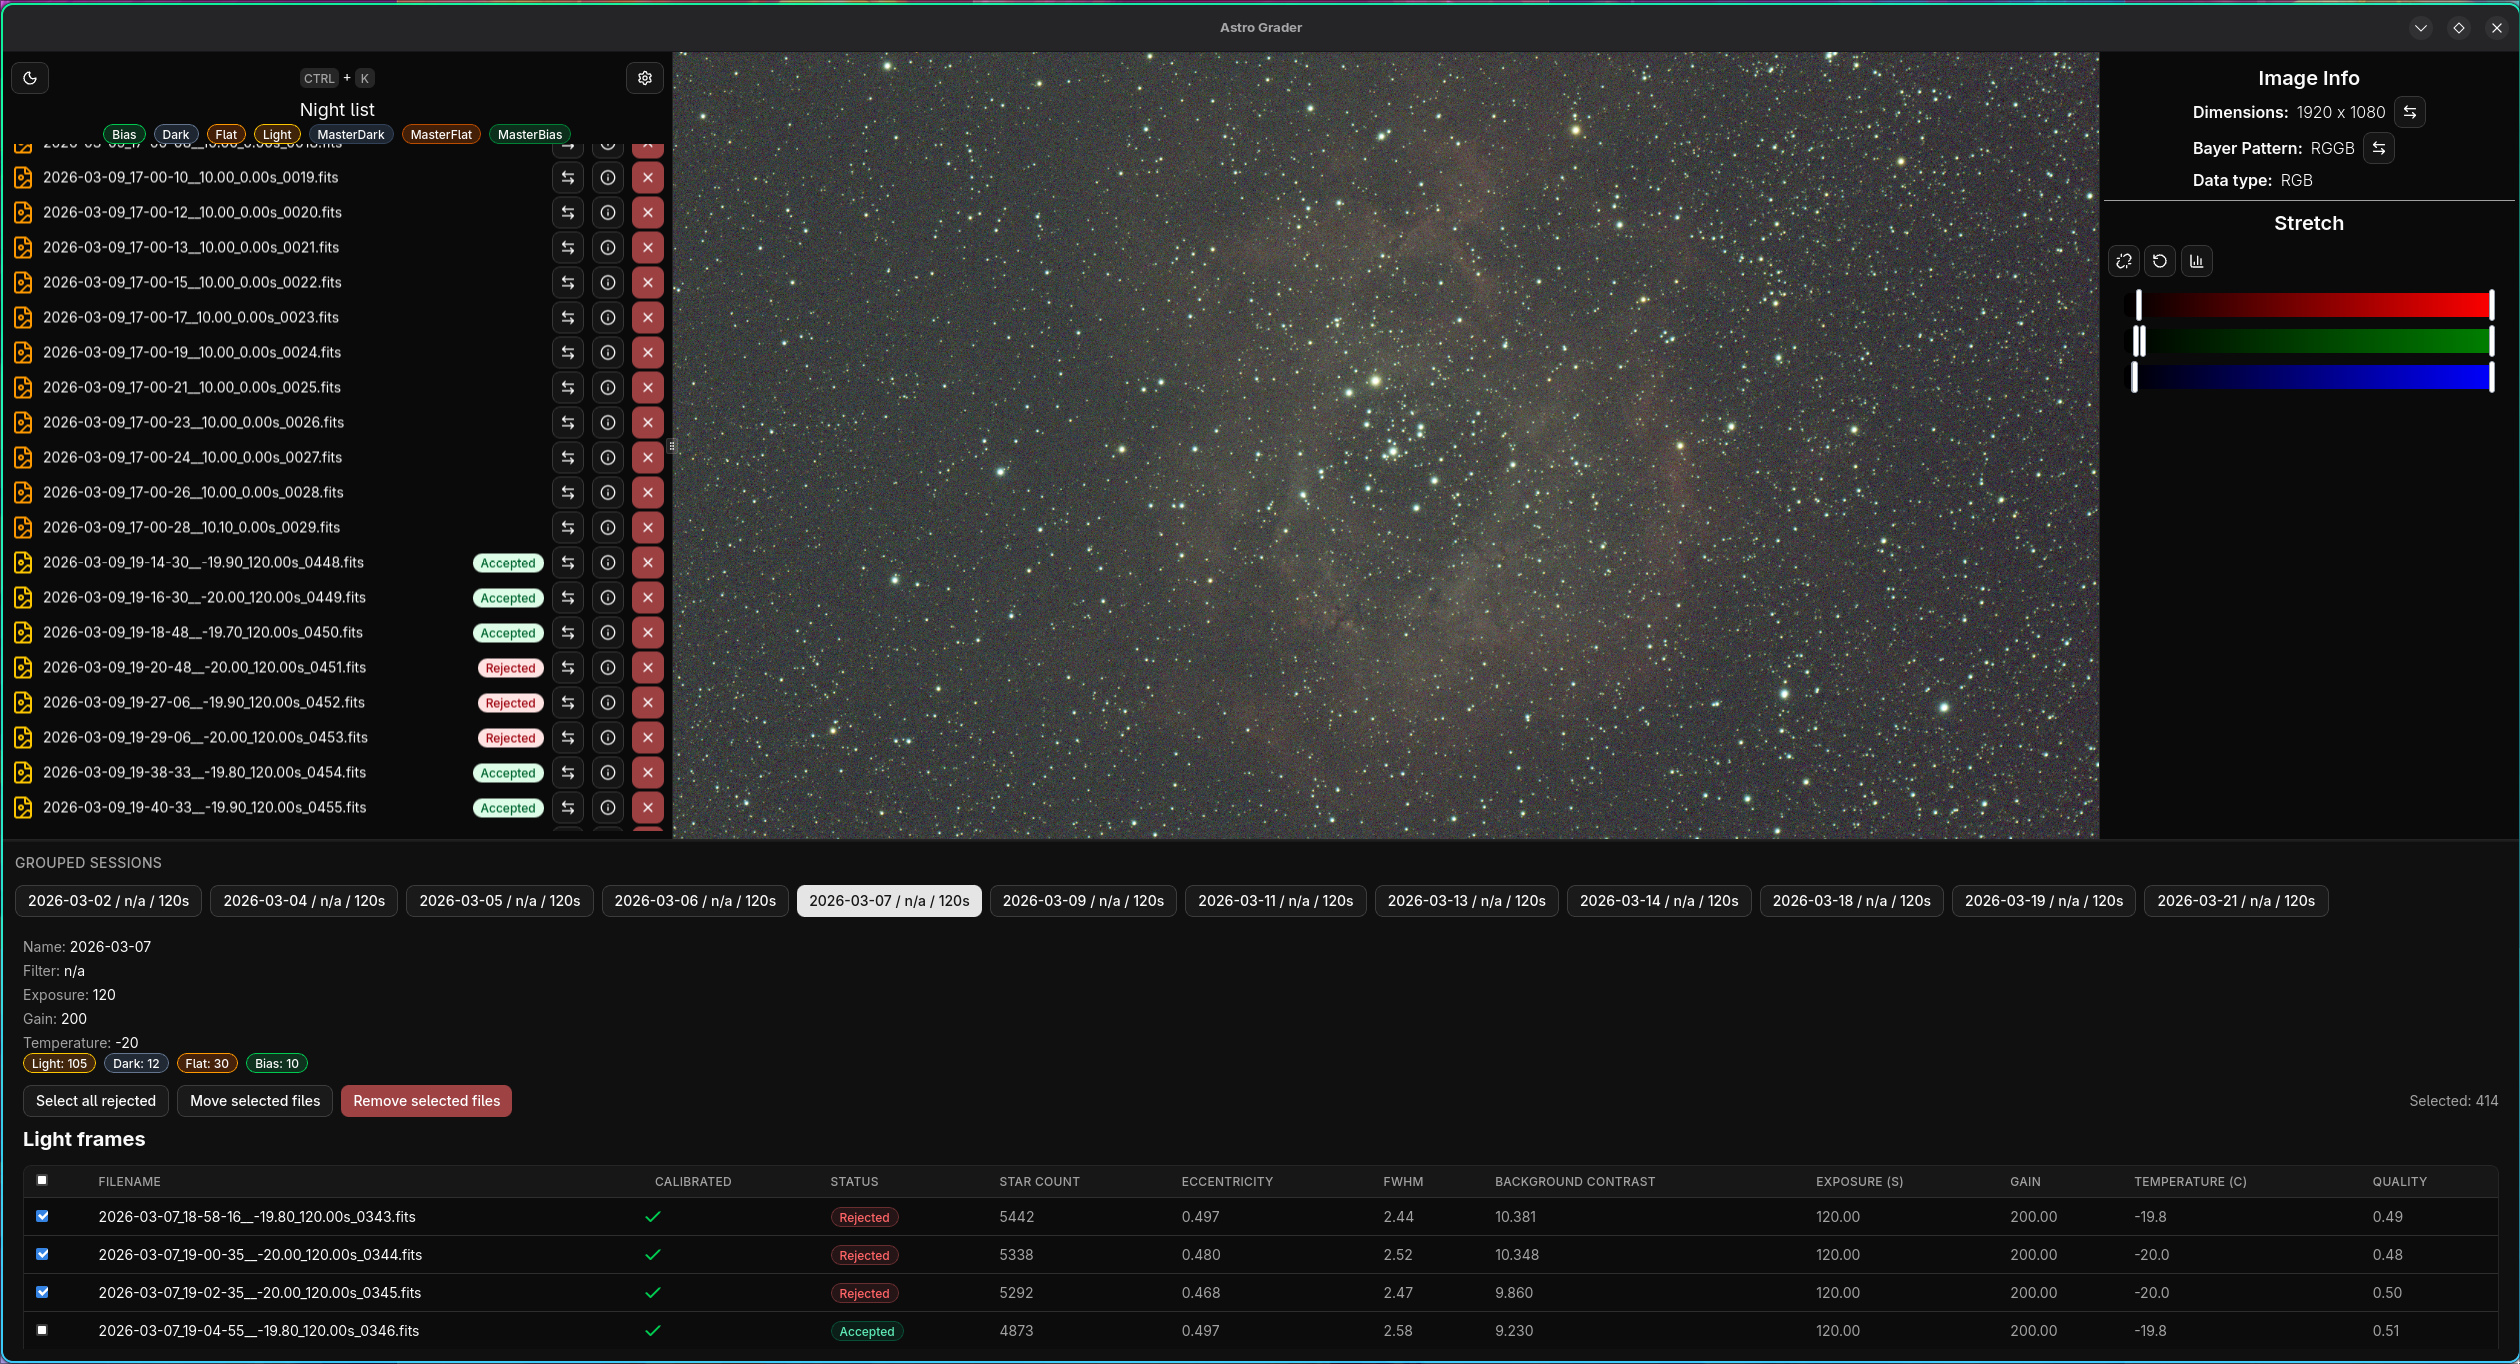
\includegraphics[width=0.95\textwidth]{assets/full_overview.png}
    \caption{Kompletní grafické uživatelské rozhraní vyvinuté aplikace.}
    \label{fig:full_ui_screenshot}
\end{figure}

\section{Výkonnostní analýza a limity diskových operací}
Pro exaktní ověření propustnosti systému byl v rámci testování využit reálný astrofotografický dataset emisní mlhoviny Rozeta (\textit{Caldwell 49 / NGC 2244}) čítající celkem 1104 surových snímků. Testovací proces zahrnoval kompletní kalibrační řetězec, tedy matematické sloučení desítek dílčích snímků plochého pole (\textit{Flat}), temných snímků (\textit{Dark}) i ofsetů (\textit{Bias}) do příslušných referenčních předloh, následnou aplikaci pixelové aritmetiky na snímky a finální extrakci profilových metrik.


Celkový čas zpracování této sady činil 32 minut. Z podrobné profilace výpočetního času vyplynulo, že samotná kalibrační fáze zabrala 30 minut, což představuje majoritní režii celé pipeline. Přestože matematické výpočty nad maticemi pixelů probíhají masivně paralelně, výpočetní vlákna jsou zásadně limitována synchronním charakterem diskových operací. V současné implementaci totiž každé vlákno v rámci své rutiny sekvenčně provádí načtení surového souboru z disku, jeho kalibraci v paměti a okamžitý zápis výsledku zpět na trvalé úložiště. Procesorový čas je tak degradován čekáním na dokončení I/O operací diskového subsystému.

Jako budoucí optimalizační krok se proto jeví restrukturalizace kalibračního modulu do architektury typu producent-konzument (\textit{Producer-Consumer}). Tento model předpokládá vyčlenění dedikovaných asynchronních vláken určených výhradně pro sekvenční čtení surových dat do sdílené paměťové fronty a paralelní zápis hotových souborů z výstupní fronty na disk. Výpočetní jádra by tak byla kontinuálně saturována čistě matematickými transformacemi pixelů bez blokování I/O operacemi, což by dramaticky zkrátilo celkovou časovou náročnost u extrémně rozsáhlých datových sad.

\section{Kritické vyhodnocení úspěšnosti hodnotících algoritmů}
Z hlediska detekce fatálních geometrických a atmosférických vad v obrazových datech vykazuje navržený deterministický aparát vysokou míru spolehlivosti. Snímky, které jsou znehodnoceny úplným zacloněním oblačností (vedoucím k poklesu počtu detekovaných hvězd pod kritickou mez) nebo závažnými chybami v chodu montáže (projevujícími se protažením profilů hvězd do stop), jsou systémem spolehlivě identifikovány a automaticky vyřazovány.

Limitace lineární kombinace skalárních statistik se však projevují při specifických atmosférických jevech, jako je přechod nízké, poloprůhledné oblačnosti či vysokého závoje. V těchto situacích dochází k dramatickému útlumu difuzního světla z hlubokého vesmíru, což vede k téměř kompletní ztrátě slabých struktur emisních mlhovin v mezihvězdném pozadí. Bodové zdroje s vysokým vlastním jasem (hvězdy) však přesto dokážou touto vrstvou prostoupit s dostatečným odstupem signálu od šumu, což segmentačnímu algoritmu stále umožňuje jejich úspěšnou extrakci. 

V důsledku matematické zranitelnosti implementovaného modelu výpočtu kontrastu pozadí, který v těchto hraničních stavech nedokáže dostatečně penalizovat plošnou ztrátu transparentnosti mikrokontrastu mlhoviny, systém takto degradované snímky chybně klasifikuje jako vyhovující a propouští je do dalšího zpracování.

Tento jev jasně ilustruje Obrázek~\ref{fig:score_comparison}. Při srovnání dvou expozic se shodně vypočteným relativním skóre $0.5$ je patrné, že pevně stanovené váhové koeficienty nedokážou flexibilně kompenzovat vzájemnou korelaci mezi jasem pozadí a lokální transparentností. Jeden ze snímků vykazuje optimální strukturální data, zatímco druhý je pro finální skládání vědeckých dat nepoužitelný. Nutnost neustálého manuálního ladění (\textit{tweakingu}) prahových hodnot pro různé typy oblohy a snímačů potvrzuje limity čistě matematického modelování a tvoří klíčový argument pro přechod k metodologické fázi hlubokého učení.

\begin{figure}[htbp]
    \centering
    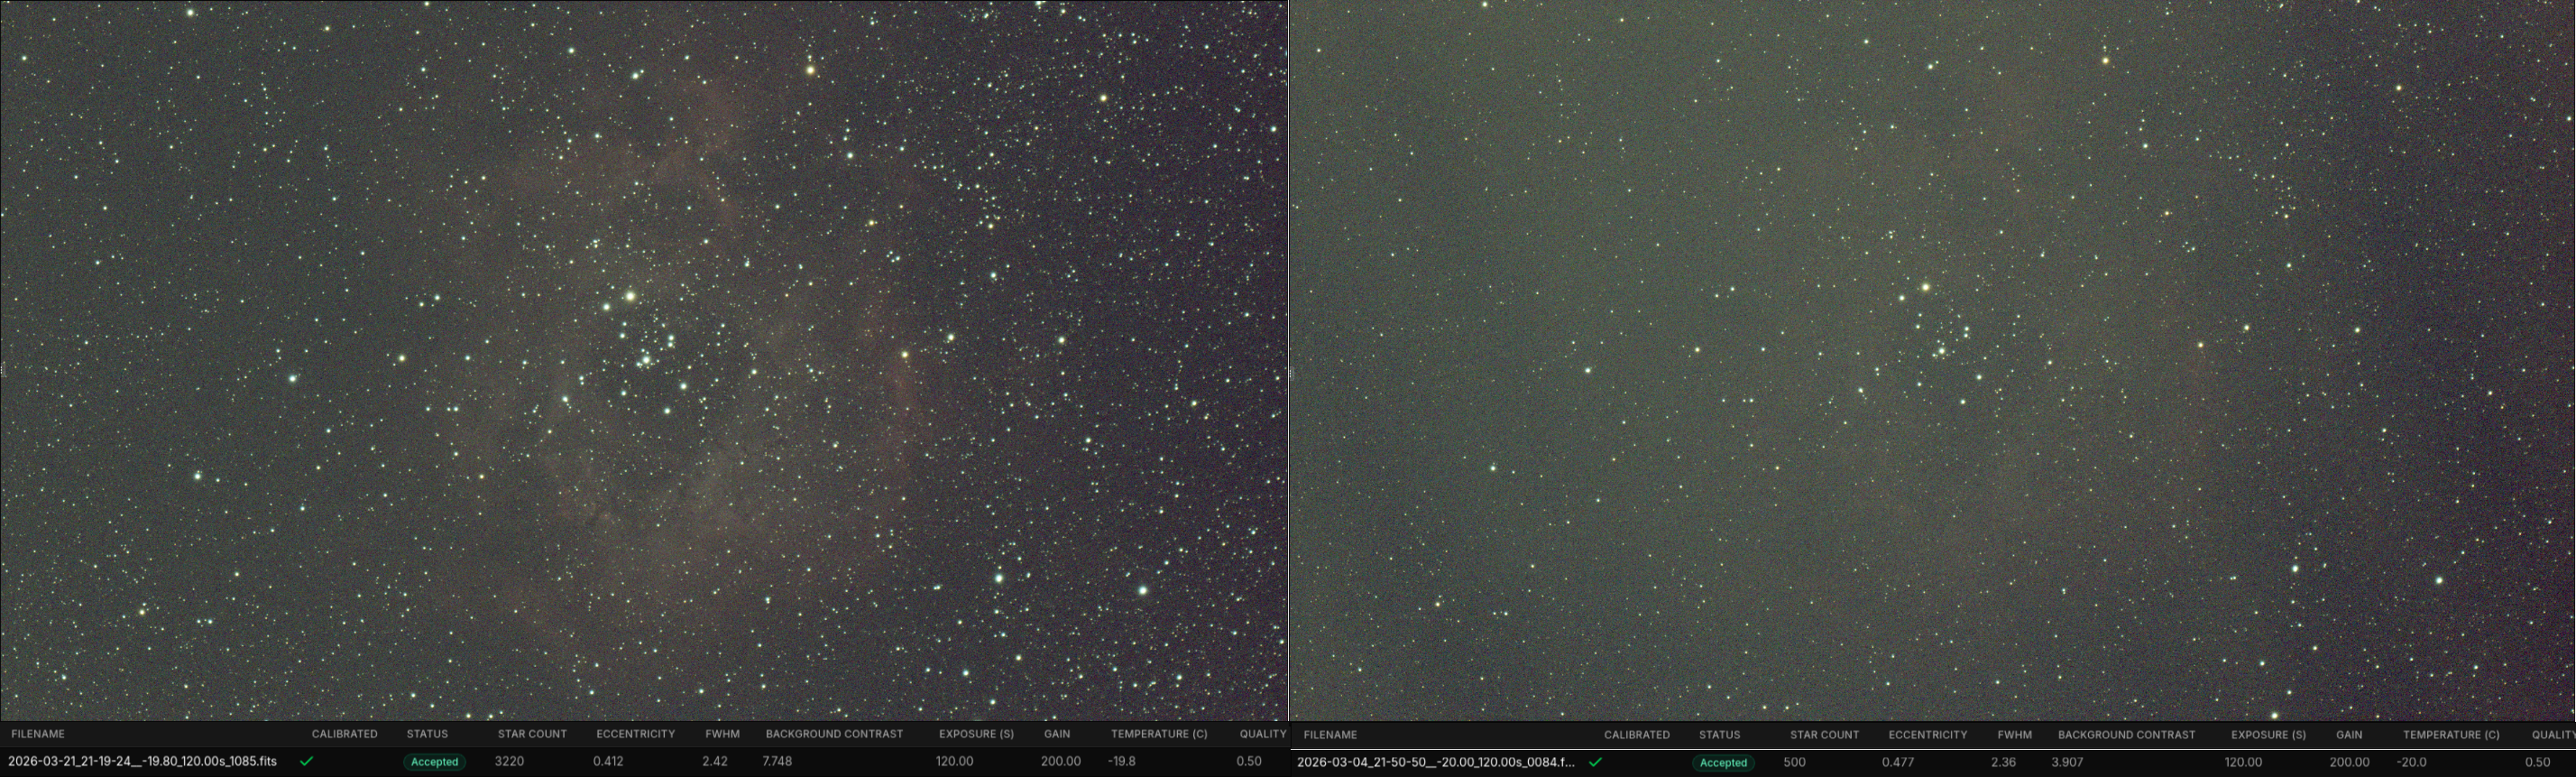
\includegraphics[width=1.0\textwidth]{assets/score_comparison.png}
    \caption{Srovnání dvou expozic se shodným vypočteným skóre (0.5)}
    \label{fig:score_comparison}
\end{figure}

Navzdory těmto drobným limitacím v hraničních oblastech systém jako celek funguje stabilně a poskytuje objektivní, reprodukovatelná data. Po mírné dodatečné korekci vah je systém plně připraven plnit svou primární roli, kterou je rychlé generování autoritativních anotačních štítků pro přípravu tréninkových dat.

\section{Návaznost na diplomovou práci a integrace neuronových sítí}
Zjištěná závislost deterministického přístupu na empirickém ladění prahových hodnot tvoří logický most k navazující diplomové práci. Cílem druhé fáze projektu bude kompletní nahrazení stávajícího statistického rozhodovacího bloku vlastním modelem hlubokého učení. 

Dokončená desktopová aplikace bude v této nadcházející etapě využita jako expertní anotační prostředí. Uživatelsky schválené, revidované a vyřazené snímky z testovacích relací poslouží jako validovaná tréninková množina. Vývojový plán předpokládá integraci tréninkového rozhraní přímo do klientské vrstvy SvelteKitu. To umožní koncovému uživateli provádět lokální jemné doladění (\textit{fine-tuning}) lehké konvoluční neuronové sítě (\ac{CNN}) přímo na specifické optické vady, vinětaci a fixní šumové charakteristiky jeho konkrétní hardwarové sestavy, čímž se zcela odstraní nutnost jakéhokoliv manuálního nastavování matematických limitů.